\chapter{Background}
\label{chap:background}

In this chapter we are going to explain the most important concepts of the 
upcoming 5G standard, talking about the Virtual Network Functions (VNFs) and 
how first experiments with this new technology already begun. Finally we are 
going to briefly introduce and explain the technologies involved and their role.

\section{Virtualization}
Cloud computing is nowadays one of the cutting edge Internet technologies, and
it is possible thanks to virtualization, that allows to isolate applications,
optimizing the utilization of hardware resources and providing more flexibility.
Virtualization, in computing, usually refers to the act of creating a virtual
version of a certain asset, such as virtual computer hardware platform,
operating system (OS), storage device, or computer network
resources~\cite{liu2014research}. Conventional virtualization
(hypervisor-based) uses virtual machines: it provides strong isolation and a
complete operating system~\cite{eder2016hypervisor}. In hypervisor
virtualization every pieces of hardware required to running software is
emulated, and it is common that the hypervisor provides interfaces to access
the real hardware, for instance to access physical devices or to communicate
with the network. However all this functionalities comes to a resource
overhead~\cite{scheepers2014virtualization}. Container-based virtualization,
instead, could be a more efficient in certain context, because it does not
emulate the entire computer. A container is seen as an isolate process running
on the host, to which the Linux kernel gives a set of capabilities.

\subsection{Network Virtualization}
Virtualization, in the networking context, refers to the act of combining
hardware, software and functionalities into a virtual network. This abstraction
runs on the top of a physical network in a hyper-visor, decoupling the logical
network from the hardware one. Network virtualization allow multiple,
heterogeneous networks to cohabit, increasing the flexibility and manageability.
The idea of network virtualization came from the decoupling of the role of the
traditional ISP into two different entities: who provides the infrastructure
(InPs) and who provides the services (SPs). In that context it is possible to
aggregate resources, even from different InPs, creating a virtual network,
offering an end-to-end service~\cite{chowdhury2009network}. Most known instances
of NV are \emph{VPNs}, dedicated networks that allows the communication among
multiple sites, using private and secure tunnels, relying on the public network
such as Internet. Other examples of network virtualization are \emph{overlay
  networks}. They are logical networks, build on the top of an existing physical
network, typically implemented at the application layer.

\section{Software-defined networking}
The SDN is an emerging approach to cloud computing and networking technology
capable of supporting the dynamic nature of future network functions and
intelligent applications while lowering operating costs through simplified
hardware, software, and management~\cite{sezer2013we}, that allows to configure
network in a programmatically way, possibly enhancing monitoring and
performances. One of the main principles of SDN architecture is to decouple the
packet forwarding process, \emph{data plane}, from the routing one, the so
called \emph{control plane}. The architecture also contemplate that network
intelligence and state are logically centralized~\cite{fundation2012software}. 

It has some drawbacks in terms of security, scalability and elasticity, because
of the centralized architecture.

\subsection{SDN stack}
\begin{figure}[ht]
 \centering
 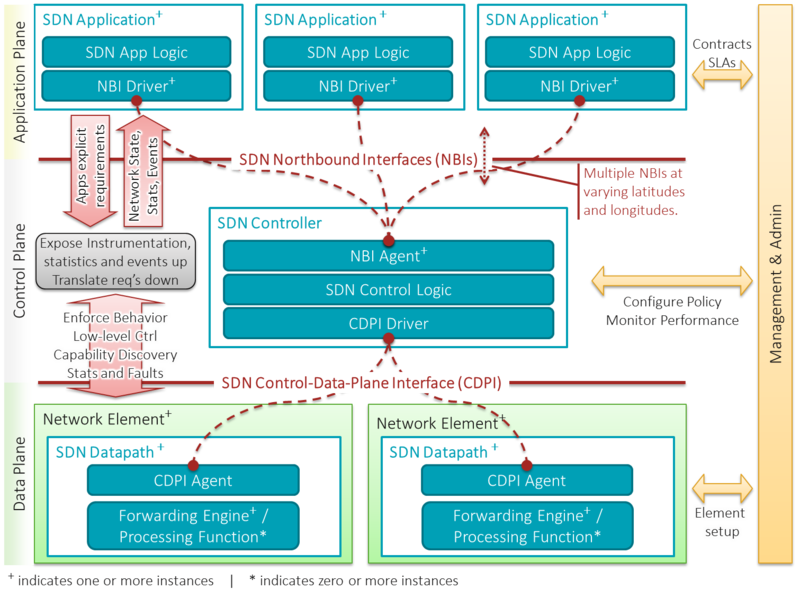
\includegraphics[scale=1.3]{sdn_architecture}
 \caption[SDN architecture schema]{SDN architecture schema. Is possible to 
denote the three layer logic: the Application plane, the Controller plane and 
the Data plane~\cite{fundation2013software}.}
 \label{chap:background:img:sdn_architecture}
\end{figure}
As depicted in Figure~\ref{chap:background:img:sdn_architecture} the SDN
architecture can be split in three different layers, also known as planes,
based on their functionalities~\cite{fundation2012software} as explained
in~\cite{fundation2013software}.

\subsubsection{Application plane}

In the \emph{Application plane} lays \emph{SDN applications} that are programs
whose role is to set the behavior of the SDN controllers 
and manage its hardware resources and data through APIs, often called 
\emph{northbound interfaces} (NBI). In order to do so they can also build an
abstracted view of the network, using controllers information, in order to make
the traffic analysis easier and to simplify the decision making process.
These interfaces provide an additional abstraction layer that high-level 
applications can consume, enabling the possibility to use a variety of 
different vendors' controllers in the same way. Applications consists both of
the two defined layers, one that is responsible to manage the whole logic, and
another one dedicated to the communication part, that in particular uses the
previously defined NBIs.

\subsubsection{Controller plane}

\emph{SDN controllers} are logically centralized components that
receive requests from SDN applications and either translate them 
in a fashion that can be understood from the SDN Datapath, or collect 
data as statics and events needed by the application to build an abstract view
of the network. 
Due to the variety of tasks a controller has to accomplish, its logical 
subdivision is achieved with a three-layer architecture, in which every layer 
exposes its own interface, that can be consequently used by the upper 
layers, up to the \emph{NBI agents}.
NBI agent manages the communications with SDN applications, exposing interfaces
to access network data and to the set of the controller functionalities.
In particular, the middle layer represents the \emph{SDN Controller Logic},
which process the requests coming from the upper layer applications. Finally
requests are communicated to the remaining network components, exploiting the
Control to Data-Plane Interface driver.

Despite the centralized design of controllers there are no limitations on the
implementation, so it possible to create federations of controllers or organize
them into a hierarchy.

\subsubsection{Data plane}
In the lowest plane we can find the \emph{SDN Datapath}, defined as a logical
network device, which exposes the possibility to access and control to its
forwarding and processing capabilities. It is composed by a CDPI agent and a set
of one or multiple traffic forwarding engines and of a zero or more traffic
processing functions that are, as a matter of fact, the devices logic. Datapath
can be mapped either to a single physical device or multiple ones and the
implementation of the its logic does not preclude neither the virtualization or
the sharing of physical resources nor the interoperability with non-SDN
networking.

\subsection{OpenFlow protocol}
The SDN strategy is often associated with the OpenFlow protocol because it is
the first standard communications interface defined between the control and the
datapath in SDN architecture~\cite{fundation2013software}, making possible to
access from controller the components of infrastructure, such as switches and
routers. OpenFlow enables the remote administration of networks working on 
layer 3: packets forwarding tables can be modified relying on packet matching 
rules. Following this approach it is possible to change routes periodically or 
ad-hoc, based on packet types, traffic or network load.

\begin{figure}[t]
 \centering
 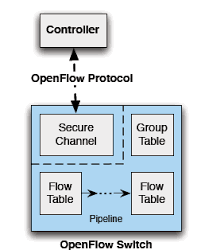
\includegraphics[scale=0.65]{openflow}
 \caption{OpenFlow protocol communication graph}
 \label{chap:background:img:openflow_protocol}
\end{figure}

In Figure~\ref{chap:background:img:openflow_protocol} it is possible to see the
how switches works in the OpenFlow protocol. Basically, OpenFlow switches own a
set of tables to organized packet control and forwarding. These tables can be
updated by higher-level application, usually an SDN application or controller,
taking advantage of OpenFlow channels (called OF channels). 

\section{Network slicing}
A network slice can be defined as a logical virtual network, tailored for a
given use case, on the top a common network using technologies such as
Software-Defined Networking and Network Function Chaining that allows network
softwarization~\cite{ordonez2017network}. The notion of separated virtual
networks deployed on the same infrastructure is not new, e.g. VPN, but it has
some specifics that make it a novel idea. The concept of network slicing was
first introduced in 2002 in~\cite{peterson2003blueprint}, where a network 
overlay that allows services to run continuously and to access the overlay
resources across different slices was illustrated.
Services operating over the overlay management have their own slice instead.
This idea was lately refined in 2016, where the design of network slicing was
based on a three-layers model~\cite{alliance2016description}, as depicted in 
Figure~\ref{chap:background:img:network_slicing}.

\begin{figure}[t]
  \centering
  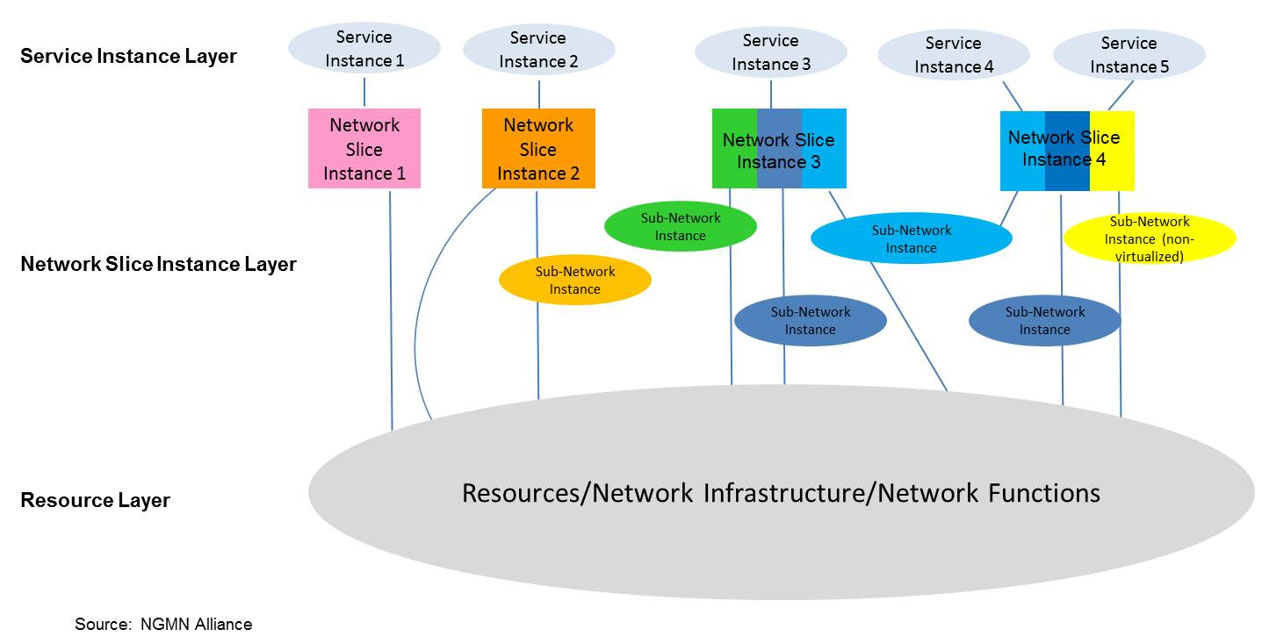
\includegraphics[scale=0.2]{networkslicing}
  \caption[The three layers model of network slicing]{The three layers model of
    network slicing~\cite{alliance2016description}}
  \label{chap:background:img:network_slicing}
\end{figure}

The first layer is the \emph{Service Instance Layer} used to represent the
business or user services supported, the second one is the \emph{Network Slice
Instance Layer}. This is a set of network functions that allows to
satisfy certain requirements~\cite{kotulski2017end}. Network functions, in
general, can be both physical, thus a combination of vendor-specific hardware
and/or virtualized. In that case the function is implemented as software and it
is decoupled from the hardware on which it is running on. Each instance must be
isolated, in order to ensure that function running at the top of it will always
provide the same Quality of Service, without degrading because of a change on
another slice~\cite{richart2016resource}. It also allows to provide better
security. In fact, in case of attack or fault of a certain slice, others must
not be affected. Moreover, each slice must implement its own set of security
function to preventing unauthorized access. Furthermore, isolation let to
manage individually each slice~\cite{ordonez2017network}. Network slice
instances are defined by a \emph{Network Slice Blueprint}: a complete
description of the structure and data flows that allow the creation and the
control of the Network Slice Instance during its whole lifecycle. The blueprint
also refers to the resources needed to assemble the network slice and defines
its characteristics (e.g. ultra-low latency, ultra-reliability, value-added
services for enterprises, etc.). The last layer is the \emph{Resource Layer},
containing both physical and logical resources, that involve all physical
assets and resources for computation, storage or transport, including radio
access.


\subsection{Network Function Virtualization}
The \emph{Network Function Virtualization} (NFV) concept refers to the use of
virtualization technologies to virtualize network nodes functions. This emerging
technology focuses on the decoupling of function logic and hardware, allowing
VNFs to run on the top of servers, switches, storage devices or on cloud
computing infrastructures. In other words the software logic is separated from
the custom platform on which it runs, enabling the use of commodity
hardware~\cite{gray2016network}. That approach worked well in the past, because
of the need to follow rigorous standards, providing at the same time high
quality, but it led to long product cycles and high specialized services that
use a combination of software and hardware resources, typically vendor-specific,
and only largely non-interoperable within other vendor solutions. New Internet
scenarios, that include IoT and the increasing number of services to spread
multimedia data (Skype, Netflix, Spotify, \dots), requires more flexible
functions and faster network deployments. This detachment provides greater
flexibility to scale VNF based on traffic and performances and also improve the
automation of function deploy and update: removing dedicated hardware also will
reduce costs machines and for maintenance.

The NFV technology is exploited in a framework, organized
at least by three components~\cite{etsi2013gs}, as represented in
Figure~\ref{chap:background:img:etsi_arch}:
\begin{enumerate}
  \item a software, able to run on over the NFVI, that performs the network
  function that must be deployed, that is the VNF;
  \item NFV Infrastructure (NFVI) that is composed by all physical resources
  and how these can be virtualized, that forms the environment where the VNFs
  are deployed;
  \item NFV MANagement and Orchestration (NFV-MANO) that covers the
  orchestration and management of both physical and logical resources, the
  functional blocks, data repositories used by these blocks, reference points
  and interfaces through which these functional blocks exchange
  information for the purpose of managing and orchestrating NFVI and VNFs.
\end{enumerate}

\begin{figure}
  \centering
  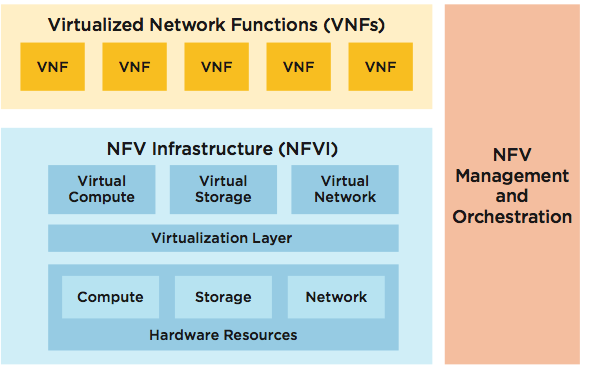
\includegraphics[scale=2]{etsi_arch}
  \caption[Network Function Virtualization reference architecture]{Network
    Function Virtualization reference architecture~\cite{etsi2013gs}}
  \label{chap:background:img:etsi_arch}
\end{figure}

\subsection{Network Function Virtualized Infrastructure}
As mentioned before, NFVI is the combination of physical and logical resources,
that combined together create the environment on which the VNFs are deployed
and run. Physical supplies can be proprietary systems, commercial-off-the-shelf
hardware, software and network resources or cloud computing capabilities. The
abstraction of resources is made taking advantage of a virtualization layer,
that hides the underlying infrastructure. Storage and computing resources may
be represented in terms of virtual machines or
containers~\cite{mijumbi2016network}.

\subsection{NFV MANagement and Orchestration}
The MANO, represented in Figure~\ref{chap:background:img:etsimano}, can be
splitted into three logical functional components:
\begin{itemize}
  \item the virtual infrastructure manager (VIM);
  \item the VNF Manager (VNFM);
  \item the NFV Orchestrator (NFVO).
\end{itemize}
And into four data repositories:
\begin{itemize}
  \item Network Service (NS) catalog;
  \item VNF catalog;
  \item NFV instances;
  \item NFVI resources.
\end{itemize}

\begin{figure}
  \centering
  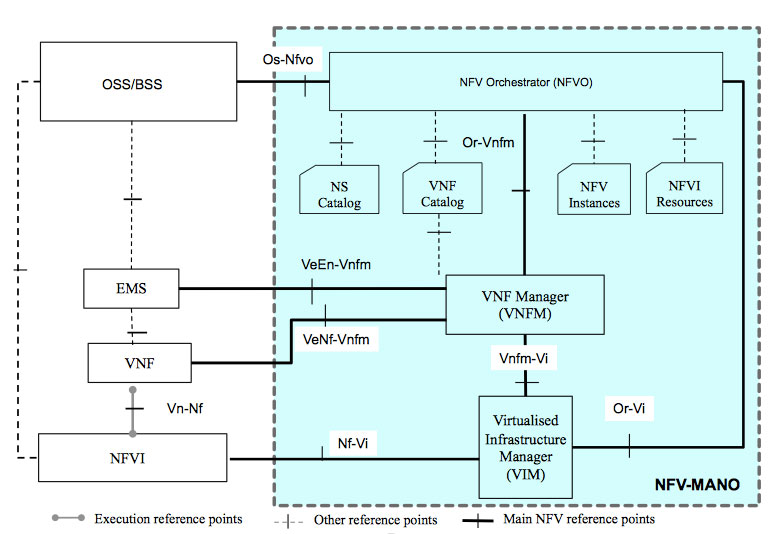
\includegraphics[scale=0.3]{etsimano}
  \caption{NFV MANO components}
  \label{chap:background:img:etsimano}
\end{figure}


\paragraph*{VIM}
The VIM aim is to manage and control NFVI resources. Every MANO can contain more
VIM instances, each of them control NFVI resources from a single infrastructure.
VIM can be developed either to administer one type of NFVI or more. VIM have to
monitor the allocation of virtual resource in order to orchestrate allocation,
upgrade, release, and reclamation of resources and optimize their usage,
including virtual links, networks, subnets, and ports. It is also the component
in charge to manage security group policies to ensure access control. In
addition, VIM also has to record data on performance and faults, that can be
queried. Thank to this component it is possible to dynamically allocate
resource, based on demand, that is particularly using IaaS.

\paragraph*{VNFM} 
In this framework all VNFs, once created, have to register to a VNFM. This
component is accountable to manage their lifecycle, that consists of
instantiation, scaling, termination and, possibly, update/upgrade, and
communicate the state of a certain VNF to others MANO blocks: this enable the
monitoring of key performance indicators (KPI), that can help to make decision
on VNF scaling. VNFM can manage a single type of VNF instances or multiple.

\paragraph*{NFVO}
The NFVO is responsible of combining functions to create end-to-end services.
Its functionalities are to ensure there are adequate compute, storage, and
network resources available to provide a network service independently of the
VIM and the creation of end-to-end services by composing different VNFs, that
can be deployed on different point-of-presence and registered to different VNF.
It also managing the topology of these services. 

\paragraph*{Data repositories} Data repositories are use to keep information on
the NFV MANO. The NS catalog is a set of predefined templates, which define
services, functions involved and their connectivity. The VNF catalog is,
instead, a set of templates describing the deployment and characteristics of
VNFs. The NFVI resources repository holds information about available/allocated
NFVI resources. The NFV instances repository keep information about functions
and services instances during their lifetimes.

\subsection{VNF challenges}
This new concept open a plethora of challenges~\cite{han2015network}. Regarding
performances, functions running on general purposes servers cloud affect
throughput and latency, moreover the capacity of the virtualized function can be
less than the hardware and software version. To reach comparable levels in terms
of performances efficient algorithms are needed, as a excellent resource
management. Another problems is the VNF management. In case of hardware
functions resources are almost equivalent, at the contrary, virtualized ones
could have costs and values that differs significantly depending on the point of
presence on which are deployed. On the other hand, since VNFs are software
components, they can elastically scale up and down, depending on the traffic
loads and user demand. Another management challenge refers to keeping track
where the VNF is running, that is of paramount importance in case of issues.
Related to possible dysfunctions, software function must reach a certain level
of reliability. Generally, purpose-build network equipment can ensure the
five-nines reliability requirement, that is more challenging to follow in that
scenario due to the higher number of possible points of failure, such as during
the scaling operation or VNF migrating from a point of presence to another.
Finally even security must be taken into account. In fact, infrastructure on
which VNFs run can be outsourced to third parties. Furthermore, orchestration
and management components must implement some sort of intrusion prevention and
detection system and the sharing of resources can introduce security threads.

\section{Service Function Chaining}
The Service Function Chaining (SFC) concept was defined
in~\cite{halpern2015service} and refers to an ordered set of Service Functions
(SF) and the constraint, defined after a classification process, to packets and
flows. SF are the particular functions whose aim is the treatment of packets
received. They can work on different levels of the network layer. These
components can be implemented as virtual elements only or in a combination of a
physical and software network elements. There are no limitations on the number
of SFs running on the same network element, so in general it is possible to have
one or more functions running on the same element. SFs can be aware or not that
are part of a certain chain, in the former case they are called \emph{SFC aware}
functions, in the latter one \emph{SFC unaware}.

The lifecycle management of the chain is enabled by two emerged technologies,
software defined networking and network defined
virtualization~\cite{medhat2017service}.

\subsection{Architecture principles}
The SFC technology was though to pursue some concept. One of the most important
principles is the \emph{decoupling}. Decoupling in terms on independence on the
infrastructure and the network, so no change must be performed to the forwarding
underlying topology to deploy SFCs, and in terms of separation between packet
handling (by SFs) and forwarding. This decoupling refers even to architecture
and functions: one must be independent from the other. Another main point is the
possibility to dynamically set routes on the incoming traffic to decide the best
treatment based on its typology. The classification can occur on different point
of the chain and can be updated during the packet delivery. Finally creation,
modification and deletion of a certain SFC must not impact on the others.

\subsection{Graph view of an SFC}
An SFC can be seen as a graph in which each node is an SF and edges are the path
through which a packet have to pass through. Because of this definitions there
are no limitations on possible cycles that can occur in the chain, in case that
a certain SF has to be reapplied on the same packet, frame or flow. These
scenarios must be adequately managed to avoid endless loops. This enable even
the possibility of branching on a certain node in order to define the treatment
that has to be imposed from that point of the chain. Traffic path in the SFC
graph is managed and described by the \emph{Service Function Forwarder} (SFF)
and \emph{Service Function Path} (SFP) components. The former is the element of
the architecture responsible of traffic forwarding. The main goals are to
redirect traffic according to the SFC specified for a specific packet flow,
query the classifier if needed and manage traffic coming back from a SF. The
SFP, instead, is an indirection layer between the fully abstract notion of SFC
and the list of SF that the traffic has to traverse. It is used for dictate the
constraint specification on the path of where packets assigned to a certain
service function path must go. There are no limitations on how specific it must
be: it can specify the exact locations, identifying both the SFF and the SF, or
only give some recommendation or, for example, defining only the SFF and
demanding to it the decision on the SF instance.


The graph representation also permit to think to \emph{unidirectional} and
\emph{bidirectional} chains. An SFC is defined unidirectional if traffic can
traverse it only in one direction, so if it is composed by 3 SF, named
\texttt{SF0}, \texttt{SF1} and \texttt{SF2} in this order, traffic can only go
from \texttt{SF0} to \texttt{SF2}. On the contrary, a bidirectional SFC allows
traffic in both directions. So, having the same chain as in the previous
example, traffic can pass both from \texttt{SF0} to \texttt{SF2} and from
\texttt{SF2} to \texttt{SF0}.

\subsection{SFC Encapsulation}
In order to exchange packet and information in the SFC ecosystem, traffic is
encapsulated. The so called SFC encapsulation carries data used by the
framework to identify SFPs, but it differs from a transport encapsulation and it
is independent from the transport one: as such any transport protocol can be
exploited to forward traffic.

This encapsulation is neither supported from SFC unaware SF nor from legacy 
SF\footnote{Legacy SF refers to network function created before SFC framework}
so \emph{SFC Proxies} has to be included in this ecosystem. These components
sits the SFF and the SFs. They accept packets from the SFF and remove the
encapsulation before delivering the packet to the SFs. In a mirrored way, it
receive the result of the SF and reapplies the SFC header, in order to be
managed by the SFF and the overall system. The communication among SFFs and
proxies is the same as the SFFs and SFC aware SF.

The \emph{Network Service Header} (NSH), used by SFC environment for
encapsulation is described in~\cite{rfc8300} and it consider three main fields
as represented in Figure~\ref{chap:background:img:nshformat}: Base Header,
Service Path Header and Context Header.
\begin{figure}[H]
  \centering
  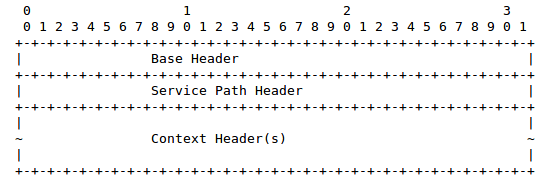
\includegraphics[scale=0.6]{nshformat}
  \caption[Network Service Header]{Network Service Header~\cite{rfc8300}}
  \label{chap:background:img:nshformat}
\end{figure}

\subsubsection{Base header}
The Base Header utility is to provide information about the service header and
the payload protocol.

\begin{figure}[H]
  \centering
  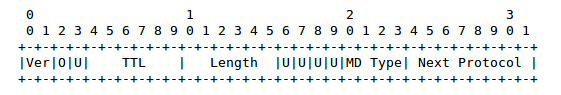
\includegraphics[scale=0.6]{nshbase}
  \caption[Network Service Header]{Network Service Header~\cite{rfc8300}}
  \label{chap:background:img:nshformat}
\end{figure}

Fields are:
\begin{description}
  \item[Version:] This field is used to set the version of the header, used for
  ensuring backward compatibility through different NSH definitions;
  \item[0 bit:] Bit set only in case of orchestration or management packets, and
  must not be changed by the SFC;
  \item[TTL:] Time To Live, indicate the maximum number of hops among SFF and
  its initial value should be configurable by the control plane. At each hop it
  must be decremented to 1 until 0: in the latter case the packet must be
  discarded. The default value is 63. This field is useful in loop prevention
  mechanism. The default value is 63;
  \item[Length:] the total length of the header (in 4-byte words), including
  the \texttt{Fixed-Length Context Header} in NSH type 0x1 or the
  \texttt{Variable-Length Context Header} in NSH type 0x2. In case of variable
  length header data must be padded to a multiple of 4;
  \item[Unassigned bits:] unassigned bits for future usages;
  \item[MD:] Metadata Type, indicate the type of the NSH. Values that now
  accepted are \texttt{0x0} that is a reserved value and if set the packet must
  be discarded, \texttt{0x1} indicate that context header length is
  fixed~\ref{subsubsec:background:flch}, \texttt{0x2} indicate that context
  header length is variable~\ref{subsubsec:background:vlch} and \texttt{0xF} for
  testing purposes (if not part of the experiment the packet must be discarded).
  Base header length and Service Path Header have always the same size;
  \item[Next Protocol:] indicates the protocol type of encapsulated data
  (protocols codes can be found at~\cite{rfc8300}).
\end{description}

\subsubsection{Service Path Header}
Provides path identification and location within a service path.

\begin{figure}[H]
  \centering
  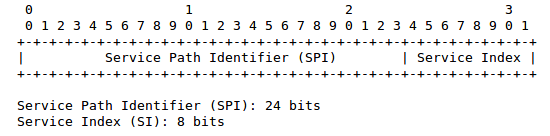
\includegraphics[scale=0.6]{nshservicepath}
  \caption[NSH Service Path Header]{NSH Service Path Header~\cite{rfc8300}}
  \label{chap:background:img:nshpath}
\end{figure}

\begin{description}
  \item[Service Path Identifier (SPI):] 24 bits, identify unambiguously an SFP.
  The first classifier have to set it;
  \item[Service Index (SI):] 8 bits, provide location within the SFP. Initially
  must be set to 255 and it must be decremented on each hop.
\end{description}

SPI combined to SI determine the next SF on each link in the chain. SI change
provide a minimal loop prevention mechanism.

\subsubsection{NSH with Fixed-Length Context Header}
\label{subsubsec:background:flch}
The NSH of type \texttt{0x1} have a 16-Byte Fixed-Length Context Header that
can be used to share data along the service path.

\begin{figure}[H]
  \centering
  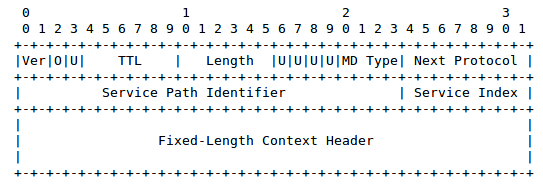
\includegraphics[scale=0.6]{nshtype1}
  \caption[NSH MD Type \texttt{0x1}]{NSH MD Type \texttt{0x1}~\cite{rfc8300}}
  \label{chap:background:img:nshtype1}
\end{figure}

The specification does not specify the content of this field and if SF or SFC
Proxy does not known its semantics they have to discard the entire packet. 

\subsubsection{NSH with Variable-Length Context Header}
\label{subsubsec:background:vlch}
In NSH of type \texttt{0x2}, zero or more Variable-Length Context Headers may
be added, but lengths must always be a multiple of 4-bytes (otherwise they must
be padded).

\begin{figure}[H]
  \centering
  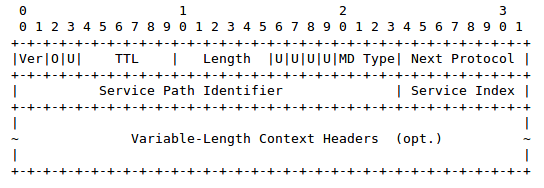
\includegraphics[scale=0.6]{nshtype2}
  \caption[NSH MD Type \texttt{0x2}]{NSH MD Type \texttt{0x2}~\cite{rfc8300}}
  \label{chap:background:img:nshtype2}
\end{figure}

The structure of the variable length part is depicted in
Figure~\ref{chap:background:img:nshtype2variable}

\begin{figure}[H]
  \centering
  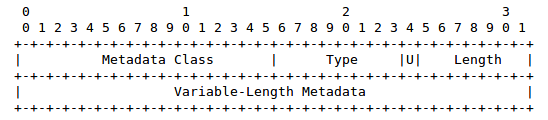
\includegraphics[scale=0.6]{nshtype2variable}
  \caption[Variable-Length Context Header]{Variable-Length Context
    Header~\cite{rfc8300}}
  \label{chap:background:img:nshtype2variable}
\end{figure}

\begin{description}
  \item[Metadata Class (MD Class):] field used in order to provide hierarchical
  namespaces for standards, vendors or other scopes;
  \item[Type:] indicates the type of metadata, depending on the MD Class;
\end{description}


\subsection{Classification of traffic}
In order to define the path of which traffic have to be forwarded, it must be
classified. The classification granularity is not specified and can occur even
during the SFC traverse. At the ingress of SFC environment packets have to be
classified to determine to choose an SFC and eventually, if the classification
granularity is too coarse, can be repeated after the treatment of some SFs. The
reclassification, also called branching, may result in a different SFP choice or
only to a metadata change.

\subsection{Other considerations}
In this architecture the SFs are viewed are resource and managed by the control
plane. Capabilities, availability and location are all accountable to the
control part as their creation. It is also in charge of collecting information
needed by the classifier to make proper decisions. The control plane could be
either distributed or centralized and even a combination is possible. 

SFC system add to the original packets information as a NSH, that both contains
metadata and information on the path that it must traverse. It is possible that
the size of the packet, in this manner, exceed the MTU on some link in the
chain. Solution must take in account this problem and the cost to overcome it.


\section{The upcoming connectivity standard: 5G}
The continuous innovation in the mobile network connectivity is leading to the
creation of a new standard, the 5G, which is estimated to arrive to the market
consumer in 2020~\cite{iwamura2015ngmn}. Lead by the Next Generation Mobile
Network (NGMN) alliance, a group composed by the major players in the field of
mobile connectivity, the 5G aims to offer not only at the end-user a new way to
browse the web, download and watch interactive content but also to create an
ad-hoc solution for Machine-to-Machine (M2M) data traffic, which is increasing
more than ever thanks to the spreading of IoT devices, which sensors need to 
continuously send data to servers/data-centers. Relatively to \emph{Long Term
Evolution} (LTE), 5G points to have data rates $10$ times better, with $10$
times smaller end-to-end latency and an increased connection density by $100$ 
times~\cite{alliance20155g}.

\begin{table}[t]
\centering
\resizebox{\textwidth}{!}{%
  \begin{tabular}{p{4,5cm}|p{5,5cm}|p{5cm}}
\textbf{Attribute}                                                    & 
\textbf{LTE capability}                                                         
 
                                                                           & 
\textbf{Improvement needed to meet NGMN requirements}                 \\ \hline
\textbf{Data rate (per user)}                                         & Up to 
100 Mb/s on average Peaks of 600 Mb/s (Cat 11/12).                              
 
                                                                     & 10X 
expected on average and peak rates and 100X expected on cell edge \\
\textbf{End-to-end latency}                                           & 10 ms 
for two-way RAN (pre-scheduled). Typically, up to 50 ms end-to-end if other 
factors are considered (e.g., transmission, CN, internet, proxy servers). & 10X 
(smaller)                                                         \\
\textbf{Mobility}                                                     & 
Functional up to 350 km/h (for certain bands up to 500 km/h). No support for 
civil aviation.                                                                
& 
1.5X                                                                  \\
\textbf{\begin{tabular}[c]{@{}l@{}}Connection\\ density\end{tabular}} & 
Typically $\sim$2,000 active users/km2.                                         
 
                                                                           & 
100X                                                                 
\end{tabular}%
}
\caption[5G improvement over LTE]{An extract from the official 5G white paper 
illustrating the improvements of 5G relatively to LTE connections.}
\label{chap:intro:table:ltevs5g}
\end{table}

Part of the new requirements can be satisfied using a large radio spectrum with
higher frequencies. The utilization of higher frequencies, though, mean that the
radio signals can be easily disrupted by physical objects, like buildings and
many geographical elements (such as hills and mountains), clashing with the
expectation of an ever-reachable connectivity. It is here where virtualization
plays an important role. In fact, the re-design of some network components today
existing via hardware can transform a monolithic networking approach to a 
modular one, exploiting the flexibility that Virtual Network Functions 
(VNFs)\cite{moens2014vnf} can offer thanks to virtualization, closing the gap to
the use-case fulfillment defined by the NGMN alliance~\cite{iwamura2015ngmn}
which require a decreased time to set up and deploy network services
(specifically, from 90 hours to 90 minutes~\cite{networld20202014role}).

\subsection{5G architecture}

With the constraints placed on the requirements formulated by the NGMN alliance,
5G envisage a multi-layered architecture, based on three main
layers~\cite{alliance20155g}:
\begin{itemize}
\item \textbf{infrastructure resource layer}: physical resources that are 
exposed via a virtualized interface, and that can be monitored using specific 
APIs
\item \textbf{business enablement layer}: where a library of functions and
  deployment is contained, and its configuration is accessible via APIs
\item \textbf{business application layer}: layer that contains specific
  applications and services of the operator
\end{itemize}

\begin{figure}[t]
  \centering
  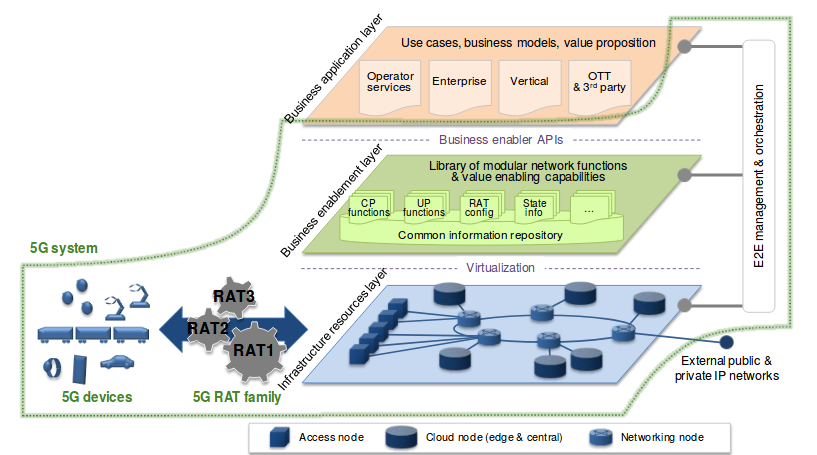
\includegraphics[scale=0.55]{5garchitecture}
  \caption[5G Architecture]{5G Architecture~\cite{alliance20155g}}
  \label{chap:background:img:5garchitecture}
\end{figure}

This separation in layers allows to easily manage multiple identities 
differently: an Internet Service Provider (ISP) could manage a multitude of 
physical infrastructures and have multiple business enablements dislocated 
along an entire continent for example, but it could decide to have only a 
single centralized business application deployment that manage all the other 
layers resources.

\subsubsection{Network slicing}
The role of a \emph{network slice} in a 5G architecture is to specifically
handle the Control-plane of a particular service (e.g. smartphones traffic,
autonomous driving, massive IoT), deploying resources in a manner that assure
the required latency, security and reliability. While some very peculiar and
legacy service could require specific hardware, the common resources between
services could be shared in a virtualized way, providing auto-scaling
capabilities in services that are under heavy network pressure.

\section{The VIBES project}
This thesis started as a part of the VIBES project~\cite{vibesesa}, whose main
requirement is to enhance the performance of end-to-end IP based that involves
satellite connections. To reach this goal, the project specifications suggest to
exploit the 5G incoming technology and use the NFV-MANO architecture to perform
first packets elaboration and performance improvement and finally TCP/IP
satellite chunk optimization with the Performance Enhancing Proxy (PEP). The
VIBES project proposed five technical requirements:
\begin{enumerate}
  \item Analysis of the applicability of current and new Internet protocols in
  the proposed VNF-PEP architecture
  \item Implementation of a VNF-PEP prototype
  \item Building of a PoC test platform
  \item VNF-PEP validation and performance tests on 5G use-cases
  \item Demonstration test-bed management
\end{enumerate}

\begin{figure}[t]
 \centering
 
\includegraphics[scale=1]{vibes_logo}
 \caption{ViBeS project logo}
 \label{chap:background:img:vibes_logo}
\end{figure}

\subsection{VNF-PEP architecture and internet protocols}
VNF-PEP is the softwarization of the usual PEP technology. One of the goals of
the project is to research and include this technology in the usual VNF
ecosystem to include without change satellite communications to the SFC. The
architecture of the systems will be based on clusters of containers whose
management and orchestration will follows the ETSI MANO architecture and SDN
principles. Thanks to VNF-PEP will be possible to dynamically take decisions on
how to optimize a certain communication.

%The analysis of this topic revealed to be trivial: since internet has many
%different protocols that would become infeasible to support all of them at the
%same time, packet encapsulation present itself as the only feasible solution:
%every packet incoming in the VNFs has already been encapsulated by a generic
%packet encapsulator/decapsulator,
%\todo{Also I think that the main purpose of UDP encapsulation is not to hide 
%the protocol used on the edges but 1) use a ``quick protocol to exchange data 
%among VNFs and 2) we are hiding the path not the protocol itself. As we were 
%discussing, we are creating some sort of proxy, so the aim will be the same 
%even if we support a plethora of protocols.''} making the whole architecture 
%independent from the protocol a particular flux of data. To achieve this, 
%several solutions have been studied, and at the end packet encapsulation with 
%TCP split (for TCP sessions) have been chosen. The rationale that guided us on 
%this choice is described in Chapter~\ref{chap:vnf_ns_impl}. \todo{Update 
%reference with the section of the explanation}
%
%\subsection{VNF-PEP prototype}
%
%Since the requirement for the whole system (MANO+PEP) were too challenging, the 
%goal shifted into creating a MANO test-bed and a working NFVI, excluding PEP. 
%The VNF architecture was shaped following the container orchestrator we decided 
%to use. An more detailed architectural implementation can be found at 
%Chapter~\ref{chap:archimpl}.
%
%\vspace{0.5cm}
%
%Starting with the first step of creating a MANO able to process incoming data
%packets through VNF functions, we encountered that many networking tools already
%present in the market required some tweaking and some integration, shifting our
%goal to create a complete European Telecommunications Standards Institutes
%(ETSI) Management and orchestrator (MANO) test-bed instead, following the
%specifications suggested in the RFC 7665, thus implementing only the first three
%requisites, without digging in the satellite data flow optimization. In
%particular, we discovered how, these tools, were suitable to create ETSI MANO
%and VNFs using virtual machine or exploiting cloud technologies, while they were
%not designed with enough flexibility an integration with Docker. In the next
%chapter we are going to take a deep analysis of the cited technologies 
%(Section~\ref{chap:prjan:sec:tech}, in order to provide to the reader enough 
%context to be able to understand our design choices we are going to describe 
%later.
%
%\noindent With this in mind, we performed a requirements analysis described in
%the next chapter.\todo{This should be put at the end of the introduction.}
% 
